\documentclass[phd,oneside]{ppgccufmg}  % ou [msc] para disserta��es
																		   % de mestrado. Para propostas ou
																		   % projetos, usar [phd,project],
																		   % [msc,proposal], etc.

\usepackage[brazil]{babel}							   % se o documento for em português, OU
%\usepackage[english]{babel}					   % se o documento for em inglês
\usepackage[utf8]{inputenc}
\usepackage[T1]{fontenc}
\usepackage{type1ec}
\usepackage{graphicx}

\PassOptionsToPackage{hyphens}{url}
\usepackage[a4paper,
english,
bookmarks=true,
bookmarksnumbered=true,
linktocpage,
colorlinks,
citecolor=black,
urlcolor=black,
linkcolor=black,
filecolor=black,
]{hyperref}

\usepackage[square]{natbib}
\usepackage[ruled,vlined]{algorithm2e}
\usepackage{amsmath,amssymb}
\usepackage{color}
\usepackage[printonlyused,nohyperlinks]{acronym}

\begin{document}

% O comando a seguir, \ppgccufmg, provê todas as informações relevantes para a
% classe ppgccufmg. Por favor, consulte a documentação para a descrição de
% cada chave.

%% Um exemplo para documentos em português é apresentado a seguir:
\ppgccufmg{
	title={Protocolo para Verifica\c{c}\~ao o de Erros\\em Redes Totalmente Confi\'aveis},
	authorrev={da Camara Neto, Vilar Fiuza},
	cutter={},
	cdu={},
	university={Universidade Federal de Minas Gerais},
	course={Computer Science},
	portuguesetitle={Protocolo para Verificacao o de Erros\\em Redes Totalmente Confi\'aveis},
	portugueseuniversity={Universidade Federal de Minas Gerais},
	portuguesecourse={Ci\^encia da Computa\c{c}\~ao},
	dedication={sections/0_0_dedication},
	portugueseuniversity={Universidade Federal de Minas Gerais},
	address={Belo Horizonte},
	date={2022-06},
	advisor=[male]{Douglas G. Macharet},
	coadvisor=[male]{Mario F. M. Campos},
	ack={sections/0_1_acknowledges},
	abstract=[brazil]{Resumo}{sections/0_2_resumo},
	abstract=[english]{Abstract}{sections/0_3_abstract},
	epigraphtext={A verdade \'e o contr\'ario da mentira, \\ e a mentira \'e o oposto da verdade.}{Autor desconhecido},
	beforetoc={
		\listofalgorithms
		\chapter*{Acronyms List}

\begin{acronym}
	\itemsep=-18pt
	%a
	\acro{AI}{Artificial Intelligence}
	\acro{APF}{Artificial Potential Field}

	%b
	\acro{BIT*}{Batch Informed Trees}
	\acro{BVP}{Boundary-Value Problem}

	%c
	\acro{CAD}{Compter Assisted Design}
	\acro{CNN}{Convolutional Neural Network}
	\acro{COSPS}{Critical Obstacles and Surrounding Point Set}
	
	%d
	\acro{DCOP}{Distributed Constraint Optimization Problem}
	\acro{DMTSPN}{Dubins Multiple Traveling Salesman Problem with Neighborhoods}
	\acro{DoF}{Degrees of Freedom}
	
	%e
	\acro{ESDF}{Euclidean Signed Distance Field}
	
	%f
	\acro{FMCW}{Frequency Modulated Continuous Wave}
	\acro{FoV}{Field of View}
	
	%g
	\acro{GP}{Gaussian Processes}
	\acro{GPS}{Global Positioning System}
	\acro{GUI}{Graphical User Interface}
	\acro{GMM}{Gaussian Mixture Model}
	\acro{GTSP}{Generalized Traveling Salesperson Problem}
	
	%h
	
	%i
	\acro{IMU}{Inertial Measurement Unit}
	\acro{IR}{Infrared}
	\acro{ITV}{Instituto Tecnológico Vale}
	
	%j
	
	%k
	
	%l
	\acro{LeGO-LOAM}{Lightweight and Ground-Optimized Lidar Odometry And Mapping}
	\acro{LiDAR}{Light Detection and Ranging}
	
	%m
	\acro{MAVs}{Micro Aerial Vehicles}
	\acro{MI}{Mutual Information}
	\acro{MILP}{Mixed Integer Linear Programming}
	\acro{MRS}{Multi-Robot Systems}
	\acro{MPC}{Model Predictive Control}
	
	%n
	\acro{NBV}{Next-best-view}
	
	%o
	\acro{OMT}{Optimal Mass Transport}
	
	%p
	\acro{PoV}{Point of View}
	
	%q
	
	%r
	\acro{RADAR}{Radio Detection and Ranging}
	\acro{RRT}{Rapidly-exploring Random Tree}
	\acro{RRT*}{Optimum Rapidly-exploring Random Tree}
	\acro{ROS}{Robot Operating System}
	\acro{RTAB-Map}{Real-Time Appearance-Based Mapping}
	
	%s
	\acro{SAR}{Search and Rescue}
	\acro{SfM}{Structure from Motion}
	\acro{SLAM}{Simultaneous Localization and Mapping}
	\acro{SLSQP}{Sequential Least SQuares Programming}
	\acro{SoNAR}{Sound navigation and ranging}
	
	%t
	\acro{TDoA}{Time Difference of Arrival}
	\acro{ToF}{Time-of-Flight}
	\acro{TSDF}{Truncated Signed Distance Field}
	\acro{TSP}{Traveling Salesman Problem}
	\acro{TWR}{Two Way Ranging}
	
	%u
	\acro{UAV}{Unmanned Aerial Vehicle}
	\acro{UWB}{Ultra-Wideband}
	
	%v
	
	
	%w
	
	%x
	
	%y
	
	%z	
	
\end{acronym}
		\chapter*{Symbol List}

\begin{table}[h]
	\begin{tabular}{ll}
		$|~.~|$ 			& Cardinality of a set\\[6pt]
		$||~.~||$      		& Euclidean norm\\[6pt]
		$(a, b)$  			& Linear regression parameters\\[6pt]
		$\alpha$  			& Robot's roll pose\\[6pt]
		$\beta$  			& Robot's pitch pose\\[6pt]
		$\mathcal{B}$  		& Mesh $\hat{\mathbb{M}}$ frontiers\\[6pt]
		$C_1(p)$  			& Cost function for euclidean distance over the path $p$\\[6pt]
		$C_2(p)$  			& Traversability cost function over the path $p$\\[6pt]
		$C_3(p)$  			& Cost function for energy consumption over the path $p$\\[6pt]
		$\mathcal{C}$  		& Cluster of reachables frontiers in $\mathcal{G}$\\[6pt]
		$\mathcal{C}_{min}$ & Minimum cluster group size\\[6pt]
		$E$  				& Edges of a graph\\[6pt]
		$eps$  				& Minimum distance to create a cluster\\[6pt]
		$\mathbb{F}$  		& Collection of mesh $\mathbb{M}$ faces\\[6pt]
		$\mathcal{F}$  		& Collection of reachable frontiers\\[6pt]
		$\gamma$  			& Robot's yaw pose\\[6pt]
		$\mathcal{G}$  		& Traversability graph\\[6pt]
		$h(x, y)$			& Terrain interpolation function\\[6pt]
		$\mathcal{H}$		& Convex hull of the spherical projected points in the visibility filtering algorithm\\[6pt]
		$\mathbb{M}$  		& Reconstructed mesh of the environment\\[6pt]
		$\mu$  				& Mean of a Gaussian distribution\\[6pt]
		$n_{goal}$  		& Goal node in the traversability graph $\mathcal{G}$\\[6pt]
		$n_{start}$  		& Start node in the traversability graph $\mathcal{G}$\\[6pt]
		$N_{\mathbb{F}}(i)$ & The set of neighboring faces of face $i$ in $\hat{\mathbb{M}}$\\
	\end{tabular}
\end{table}

\begin{table}[b]
	\begin{tabular}{ll}
		$N_{\{d,t,e\}}$  	& Normalization coefficients for the combined metric different components\\[6pt]
		$o$  				& Closest non-traversable point\\[6pt]
		$\mathcal{O}$  		& Big O asymptotic notation\\[6pt]
		$p$  		& A traversable path for ground robots\\[6pt]
		$p_{global}$  		& Estimated global traversable path for ground robots\\[6pt]	
		$p_{local}$  		& Estimated local traversable path for ground robots\\[6pt]	
		$x_{sampled}$ 		& Point inside this radius closer to the target frontier \\[6pt]
		$\bar{p}$  			& Modified path $p$\\[6pt]
		$P_{\{d,t,e\}}$  	& Weights for the combined metric different components\\[6pt]
		$\mathcal{PC}$  	& Raw point cloud from the LiDAR sensor\\[6pt]
		$q$      			& Instant Pose of the robot $R$\\[6pt]		
		$r$  				& Random value in the range $(0, 1]$\\[6pt]
		$R$  				& Representation of a robot (real or simulated)\\[6pt]
		$\hat{\mathcal{R}}$ & Updated robot $\mathcal{R}$ pose\\[6pt]
		$\mathcal{SP}$  	& Support polygon of the robot\\[6pt]
		$sim(a, b)$  		& Similarity function based on the RMSE between two pointclouds $a$ and $b$\\[6pt]
		$\sigma^2$  		& Variance of a Gaussian distribution\\[6pt]
		$\sigma$  			& Standard deviation of a Gaussian distribution\\[6pt]
		$\mathcal{T}$  		& Octree of the map $\mathbb{M}$\\[6pt]
		$\tau_{bump}$  		& Bumpiness threshold\\[6pt]
		$\tau_{inflation}$  & Border inflation threshold in $\mathcal{G}$\\[6pt]
		$$  		&         \\[6pt]
		$$  		&         \\[6pt]
		$$  		&         \\[6pt]
		$$  		&         \\[6pt]
		$$  		&         \\[6pt]
		$$  		&         \\[6pt]
		$$  		&         \\[6pt]
		$$  		&         \\[6pt]
		$$  		&         \\[6pt]
		$$  		&         \\
	\end{tabular}
\end{table}



%\begin{table}[h]
%	\begin{tabular}{ll}
%		$$  		&         \\[6pt]
%		$$  		&         \\[6pt]
%		$$  		&         \\[6pt]
%		$$  		&         \\[6pt]
%		$$  		&         \\[6pt]
%		$$  		&         \\[6pt]
%		$$  		&         \\[6pt]
%		$$  		&         \\[6pt]
%		$$  		&         \\[6pt]
%		$$  		&         \\[6pt]
%		$$  		&         \\[6pt]
%		$$  		&         \\[6pt]
%		$$  		&         \\[6pt]
%		$$  		&         \\[6pt]
%		$$  		&         \\[6pt]
%		$$  		&         \\[6pt]
%		$$  		&         \\[6pt]
%		$$  		&         \\[6pt]
%		$$  		&         \\[6pt]
%		$$  		&         \\[6pt]
%		$$  		&         \\[6pt]
%		$$  		&         \\[6pt]
%		$$  		&         \\[6pt]
%		$$  		&         \\[6pt]
%		$$  		&         \\[6pt]
%		$$  		&         \\[6pt]
%		$$  		&         \\[6pt]
%		$$  		&         \\[6pt]
%		$$  		&         \\[6pt]
%		$$   	    & 			\\
%	\end{tabular}
%\end{table}

	},
	keywords={Robotics, Exploration, Confined spaces},
	postkeywords={Robotics, Exploration, Confined spaces},
	%approval={sections/FolhadeAprovacaoSEI_XXXX_page1.pdf},
	%approval={sections/FolhadeAprovacaoSEI_XXXX_page2.pdf},
	%fcpage={sections/ficha_catalografica_XXXX.pdf},
}

% Um exemplo para documentos em inglês é apresentado a seguir (lembre-se de
% usar \usepackage[english]{babel}):
%\ppgccufmg{
%	title={Verification protocol for totally reliable networks},
%	authorrev={da Camara Neto, Vilar Fiuza},
%	cutter={},
%	cdu={},
%	university={Universidade Federal de Minas Gerais},
%	course={Computer Science},
%	portuguesetitle={Protocolo para Verificacao o de Erros\\em Redes Totalmente Confi\'aveis},
%	portugueseuniversity={Universidade Federal de Minas Gerais},
%	portuguesecourse={Ci\^encia da Computa\c{c}\~ao},
%	dedication={sections/0_0_dedication},
%	portugueseuniversity={Universidade Federal de Minas Gerais},
%	address={Belo Horizonte},
%	date={2022-06},
%	advisor=[male]{Adamastor Pompeu Setúbal},
%	coadvisor=[female]{Maria Perez},
%	ack={sections/0_1_acknowledges},
%	abstract=[brazil]{Resumo}{sections/0_2_resumo},
%	abstract=[english]{Abstract}{sections/0_3_abstract},
%	epigraphtext={You should update this text.}{Unknown author},
%	beforetoc={
%		\listofalgorithms
%		\chapter*{Acronyms List}

\begin{acronym}
	\itemsep=-18pt
	%a
	\acro{AI}{Artificial Intelligence}
	\acro{APF}{Artificial Potential Field}

	%b
	\acro{BIT*}{Batch Informed Trees}
	\acro{BVP}{Boundary-Value Problem}

	%c
	\acro{CAD}{Compter Assisted Design}
	\acro{CNN}{Convolutional Neural Network}
	\acro{COSPS}{Critical Obstacles and Surrounding Point Set}
	
	%d
	\acro{DCOP}{Distributed Constraint Optimization Problem}
	\acro{DMTSPN}{Dubins Multiple Traveling Salesman Problem with Neighborhoods}
	\acro{DoF}{Degrees of Freedom}
	
	%e
	\acro{ESDF}{Euclidean Signed Distance Field}
	
	%f
	\acro{FMCW}{Frequency Modulated Continuous Wave}
	\acro{FoV}{Field of View}
	
	%g
	\acro{GP}{Gaussian Processes}
	\acro{GPS}{Global Positioning System}
	\acro{GUI}{Graphical User Interface}
	\acro{GMM}{Gaussian Mixture Model}
	\acro{GTSP}{Generalized Traveling Salesperson Problem}
	
	%h
	
	%i
	\acro{IMU}{Inertial Measurement Unit}
	\acro{IR}{Infrared}
	\acro{ITV}{Instituto Tecnológico Vale}
	
	%j
	
	%k
	
	%l
	\acro{LeGO-LOAM}{Lightweight and Ground-Optimized Lidar Odometry And Mapping}
	\acro{LiDAR}{Light Detection and Ranging}
	
	%m
	\acro{MAVs}{Micro Aerial Vehicles}
	\acro{MI}{Mutual Information}
	\acro{MILP}{Mixed Integer Linear Programming}
	\acro{MRS}{Multi-Robot Systems}
	\acro{MPC}{Model Predictive Control}
	
	%n
	\acro{NBV}{Next-best-view}
	
	%o
	\acro{OMT}{Optimal Mass Transport}
	
	%p
	\acro{PoV}{Point of View}
	
	%q
	
	%r
	\acro{RADAR}{Radio Detection and Ranging}
	\acro{RRT}{Rapidly-exploring Random Tree}
	\acro{RRT*}{Optimum Rapidly-exploring Random Tree}
	\acro{ROS}{Robot Operating System}
	\acro{RTAB-Map}{Real-Time Appearance-Based Mapping}
	
	%s
	\acro{SAR}{Search and Rescue}
	\acro{SfM}{Structure from Motion}
	\acro{SLAM}{Simultaneous Localization and Mapping}
	\acro{SLSQP}{Sequential Least SQuares Programming}
	\acro{SoNAR}{Sound navigation and ranging}
	
	%t
	\acro{TDoA}{Time Difference of Arrival}
	\acro{ToF}{Time-of-Flight}
	\acro{TSDF}{Truncated Signed Distance Field}
	\acro{TSP}{Traveling Salesman Problem}
	\acro{TWR}{Two Way Ranging}
	
	%u
	\acro{UAV}{Unmanned Aerial Vehicle}
	\acro{UWB}{Ultra-Wideband}
	
	%v
	
	
	%w
	
	%x
	
	%y
	
	%z	
	
\end{acronym}
%		\chapter*{Symbol List}

\begin{table}[h]
	\begin{tabular}{ll}
		$|~.~|$ 			& Cardinality of a set\\[6pt]
		$||~.~||$      		& Euclidean norm\\[6pt]
		$(a, b)$  			& Linear regression parameters\\[6pt]
		$\alpha$  			& Robot's roll pose\\[6pt]
		$\beta$  			& Robot's pitch pose\\[6pt]
		$\mathcal{B}$  		& Mesh $\hat{\mathbb{M}}$ frontiers\\[6pt]
		$C_1(p)$  			& Cost function for euclidean distance over the path $p$\\[6pt]
		$C_2(p)$  			& Traversability cost function over the path $p$\\[6pt]
		$C_3(p)$  			& Cost function for energy consumption over the path $p$\\[6pt]
		$\mathcal{C}$  		& Cluster of reachables frontiers in $\mathcal{G}$\\[6pt]
		$\mathcal{C}_{min}$ & Minimum cluster group size\\[6pt]
		$E$  				& Edges of a graph\\[6pt]
		$eps$  				& Minimum distance to create a cluster\\[6pt]
		$\mathbb{F}$  		& Collection of mesh $\mathbb{M}$ faces\\[6pt]
		$\mathcal{F}$  		& Collection of reachable frontiers\\[6pt]
		$\gamma$  			& Robot's yaw pose\\[6pt]
		$\mathcal{G}$  		& Traversability graph\\[6pt]
		$h(x, y)$			& Terrain interpolation function\\[6pt]
		$\mathcal{H}$		& Convex hull of the spherical projected points in the visibility filtering algorithm\\[6pt]
		$\mathbb{M}$  		& Reconstructed mesh of the environment\\[6pt]
		$\mu$  				& Mean of a Gaussian distribution\\[6pt]
		$n_{goal}$  		& Goal node in the traversability graph $\mathcal{G}$\\[6pt]
		$n_{start}$  		& Start node in the traversability graph $\mathcal{G}$\\[6pt]
		$N_{\mathbb{F}}(i)$ & The set of neighboring faces of face $i$ in $\hat{\mathbb{M}}$\\
	\end{tabular}
\end{table}

\begin{table}[b]
	\begin{tabular}{ll}
		$N_{\{d,t,e\}}$  	& Normalization coefficients for the combined metric different components\\[6pt]
		$o$  				& Closest non-traversable point\\[6pt]
		$\mathcal{O}$  		& Big O asymptotic notation\\[6pt]
		$p$  		& A traversable path for ground robots\\[6pt]
		$p_{global}$  		& Estimated global traversable path for ground robots\\[6pt]	
		$p_{local}$  		& Estimated local traversable path for ground robots\\[6pt]	
		$x_{sampled}$ 		& Point inside this radius closer to the target frontier \\[6pt]
		$\bar{p}$  			& Modified path $p$\\[6pt]
		$P_{\{d,t,e\}}$  	& Weights for the combined metric different components\\[6pt]
		$\mathcal{PC}$  	& Raw point cloud from the LiDAR sensor\\[6pt]
		$q$      			& Instant Pose of the robot $R$\\[6pt]		
		$r$  				& Random value in the range $(0, 1]$\\[6pt]
		$R$  				& Representation of a robot (real or simulated)\\[6pt]
		$\hat{\mathcal{R}}$ & Updated robot $\mathcal{R}$ pose\\[6pt]
		$\mathcal{SP}$  	& Support polygon of the robot\\[6pt]
		$sim(a, b)$  		& Similarity function based on the RMSE between two pointclouds $a$ and $b$\\[6pt]
		$\sigma^2$  		& Variance of a Gaussian distribution\\[6pt]
		$\sigma$  			& Standard deviation of a Gaussian distribution\\[6pt]
		$\mathcal{T}$  		& Octree of the map $\mathbb{M}$\\[6pt]
		$\tau_{bump}$  		& Bumpiness threshold\\[6pt]
		$\tau_{inflation}$  & Border inflation threshold in $\mathcal{G}$\\[6pt]
		$$  		&         \\[6pt]
		$$  		&         \\[6pt]
		$$  		&         \\[6pt]
		$$  		&         \\[6pt]
		$$  		&         \\[6pt]
		$$  		&         \\[6pt]
		$$  		&         \\[6pt]
		$$  		&         \\[6pt]
		$$  		&         \\[6pt]
		$$  		&         \\
	\end{tabular}
\end{table}



%\begin{table}[h]
%	\begin{tabular}{ll}
%		$$  		&         \\[6pt]
%		$$  		&         \\[6pt]
%		$$  		&         \\[6pt]
%		$$  		&         \\[6pt]
%		$$  		&         \\[6pt]
%		$$  		&         \\[6pt]
%		$$  		&         \\[6pt]
%		$$  		&         \\[6pt]
%		$$  		&         \\[6pt]
%		$$  		&         \\[6pt]
%		$$  		&         \\[6pt]
%		$$  		&         \\[6pt]
%		$$  		&         \\[6pt]
%		$$  		&         \\[6pt]
%		$$  		&         \\[6pt]
%		$$  		&         \\[6pt]
%		$$  		&         \\[6pt]
%		$$  		&         \\[6pt]
%		$$  		&         \\[6pt]
%		$$  		&         \\[6pt]
%		$$  		&         \\[6pt]
%		$$  		&         \\[6pt]
%		$$  		&         \\[6pt]
%		$$  		&         \\[6pt]
%		$$  		&         \\[6pt]
%		$$  		&         \\[6pt]
%		$$  		&         \\[6pt]
%		$$  		&         \\[6pt]
%		$$  		&         \\[6pt]
%		$$   	    & 			\\
%	\end{tabular}
%\end{table}

%	},
%	keywords={Robotics, Exploration, Confined spaces},
%	postkeywords={Robotics, Exploration, Confined spaces},
%	%approval={sections/FolhadeAprovacaoSEI_XXXX_page1.pdf},
%	%approval={sections/FolhadeAprovacaoSEI_XXXX_page2.pdf},
%	%fcpage={sections/ficha_catalografica_XXXX.pdf},
%}

% Os três comandos seguintes são apenas para gerar texto para ocupar espaço nas
% páginas.
\newcommand{\dummytxta}{%
Lorem ipsum dolor sit amet, consectetur adipisicing elit, sed do
eiusmod tempor incididunt ut labore et dolore magna aliqua. Ut enim ad
minim veniam, quis nostrud exercitation ullamco laboris nisi ut
aliquip ex ea commodo consequat. Duis aute irure dolor in
reprehenderit in voluptate velit esse cillum dolore eu fugiat nulla
pariatur. Excepteur sint occaecat cupidatat non proident, sunt in
culpa qui officia deserunt mollit anim id est laborum.\par
}

\newcommand{\dummytxtb}{%
Sed ut perspiciatis unde omnis iste natus error sit voluptatem accusantium
doloremque laudantium, totam rem aperiam, eaque ipsa quae ab illo inventore
veritatis et quasi architecto beatae vitae dicta sunt explicabo. Nemo enim
ipsam voluptatem quia voluptas sit aspernatur aut odit aut fugit, sed quia
consequuntur magni dolores eos qui ratione voluptatem sequi nesciunt. Neque
porro quisquam est, qui dolorem ipsum quia dolor sit amet, consectetur,
adipisci velit, sed quia non numquam eius modi tempora incidunt ut labore et
dolore magnam aliquam quaerat voluptatem. Ut enim ad minima veniam, quis
nostrum exercitationem ullam corporis suscipit laboriosam, nisi ut aliquid ex
ea commodi consequatur? Quis autem vel eum iure reprehenderit qui in ea
voluptate velit esse quam nihil molestiae consequatur, vel illum qui dolorem
eum fugiat quo voluptas nulla pariatur?\par
}

\newcommand{\dummytxtc}{%
At vero eos et accusamus et iusto odio dignissimos ducimus qui blanditiis
praesentium voluptatum deleniti atque corrupti quos dolores et quas molestias
excepturi sint occaecati cupiditate non provident, similique sunt in culpa qui
officia deserunt mollitia animi, id est laborum et dolorum fuga. Et harum
quidem rerum facilis est et expedita distinctio. Nam libero tempore, cum soluta
nobis est eligendi optio cumque nihil impedit quo minus id quod maxime placeat
facere possimus, omnis voluptas assumenda est, omnis dolor
repellendus. Temporibus autem quibusdam et aut officiis debitis aut rerum
necessitatibus saepe eveniet ut et voluptates repudiandae sint et molestiae non
recusandae. Itaque earum rerum hic tenetur a sapiente delectus, ut aut
reiciendis voluptatibus maiores alias consequatur aut perferendis doloribus
asperiores repellat.\par
}

\newcommand{\dummytxt}{\dummytxta\dummytxtb\dummytxtc}

\chapter{Introdução}

Segundo \cite{horn86robot}, todo triângulo equilátero tem os lados iguais. Já
segundo \cite{shashua97photometric}, todo quadrado também tem.

Veja que o pacote \verb|natbib| permite uma série de formas diferentes para
fazer referências bibliográficas. O comando padrão, \verb|\cite|, realiza a
citação comum vista no parágrafo anterior. Outros comandos permitem, por
exemplo, citar somente o autor --- por exemplo, citar o trabalho de
\citeauthor{samaras99coupled} --- ou colocar automaticamente a citação entre
parênteses \citep{hougen93estimation, sato99illumination2, sato99illumination1,
sato01stability}. Os comandos usados foram, respectivamente, \verb|\citeauthor|
e \verb|\citep|. Veja a documentação do \verb|natbib| na Internet para conhecer
outros comandos e exemplos de uso.

Citações aleatórias para fazer com que as referências bibliográficas ocupem
mais de uma página: \cite{bichsel92simple, dror01statistics, guisser92new}.

Para adicionar um acrônimo usar \verb|\ac{}| com o identificador do acrônimo: \ac{LeGO-LOAM}.

\section{Motivação}

\dummytxtb\dummytxta

\subsection{Sub-motivação}


\dummytxtc\dummytxtb

\subsection{Mais uma sub-seção}

\dummytxta\dummytxtc

\subsubsection{Descendo mais um nível}

\dummytxtb\dummytxta


\chapter{Desenvolvimento}

\dummytxtb\dummytxta\dummytxtc

\begin{figure}[t]
    \centering
    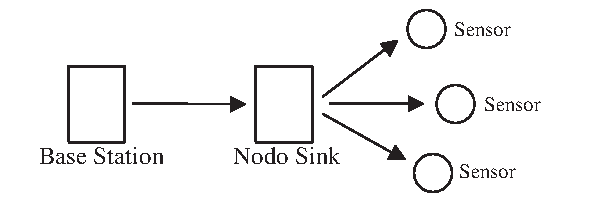
\includegraphics{img/exemplo}
    \caption{Uma figura de exemplo.}
    \label{fig:exemplo}
\end{figure}

\dummytxtb\dummytxta\dummytxtc\dummytxtb

\begin{table}[t]
    \caption{Uma tabela de exemplo.}
    {\centering
    \begin{tabular}{lcr} \toprule
    \emph{Left-aligned} & \emph{Centered} & \emph{Right-aligned} \\ \midrule
    Lorem ipsum & dolor sit & amet \\
    consectetur adipisicing & elit, sed do eiusmod & tempor \\
    incididunt ut & labore et dolore & magna aliqua. \\ \bottomrule
    \end{tabular}\par
    }
\end{table}


\begin{algorithm}
	$i\gets 10$\;
	\eIf{$i\geq 5$}
	{
		$i\gets i-1$\;
	}{
		\If{$i\leq 3$}
		{
			$i\gets i+2$\;
		}
	}
	\caption{Verificação quántica}
	\label{alg:frontier}
\end{algorithm}

% Aqui vem a parte da bibliografia: use o comando \ppgccbibliography indicando
% apenas o nome do arquivo .bib (sem a extensão).
\ppgccbibliography{bibfile}


% Este comando encapsula o conjunto de apêndices. A sua função é fazer com que
% a numeração dos apêndices seja feita com letras maiúsculas (A, B, C, etc.) e
% a palavra "Apêndice" anteceda as entradas no Sumário.
\begin{appendices}

% Para cada apêndice, um \chapter
\chapter{Um apêndice}

\dummytxta
\dummytxtb
\dummytxtc
\dummytxta
\dummytxtb

\chapter{Outro apêndice}

\dummytxta
\dummytxtb
\dummytxtc
\dummytxta
\dummytxtb

% Fim dos apêndices (usar apenas depois do último apêndice)
\end{appendices}


% Este comando encapsula o conjunto de anexos. A sua função é fazer com que a
% numeração dos anexos seja feita com letras maiúsculas (A, B, C, etc.) e a
% palavra "Anexo" anteceda as entradas no Sumário.
\begin{attachments}

% Para cada anexo, um \chapter
\chapter{Um anexo}

\dummytxta
\dummytxtb
\dummytxtc
\dummytxta
\dummytxtb

\chapter{Outro anexo}

\dummytxta
\dummytxtb

% Fim dos anexos (usar apenas depois do último anexo)
\end{attachments}


\end{document}
